% -----------------------------------------------------------------------------
% Fundamentação Teórica
% -----------------------------------------------------------------------------

\chapter{Fundamentação Teórica}
\label{chap:fundamentacaoTeorica}

Neste capítulo são discutidos conceitos fundamentais para o melhor entendimento deste 
trabalho. A primeira seção define o conceito de \textit{Big Data}, e discute como esse 
cenário impulsionou o desenvolvimento de soluções para armazenamento, e gerenciamento de 
grandes volumes de dados. Também serão analisados novos modelos de dados e sistemas de 
gerenciamento de banco de dados (SGBDs), que surgiram como alternativa para os modelos 
convencionais no contexto de \textit{Big Data}. A seção \ref{sec:spark} fala 
sobre ferramentas auxiliares, que podem ser utilizadas para processar grandes volumes de dados,
especificamente serão apresentadas as plataformas Hadoop e Spark. Por fim, a seção 
\ref{sec:api}, trata sobre \textit{web services}, soluções para comunicação entre aplicações, 
que viabilizam, por exemplo, o acesso a dados que uma ferramenta disponibiliza.

\section{Big Data e NoSQL}
\label{sec:bigdata}

A evolução tecnológica viabilizou um grande aumento na velocidade e quantidade de dados que 
são gerados diariamente. Esses dados são produzidos em transações \textit{online}, redes sociais, 
dispositivos móveis, sensores, registros governamentais, entre outros. Esse fenômeno ficou 
conhecido como \textit{Big Data} \cite{sagiroglu2013big}. 

O termo \textit{Big Data} é caracterizado por três componentes: variedade, volume e velocidade. 
O primeiro componente se refere a variedade de fontes e tipos dos dados, em geral eles 
aparecem em três tipos: estruturados, não estruturados e semiestruturados. O segundo componente 
de \textit{Big Data}, o volume, se refere a grande escala na quantidade de dados que são 
adquiridos, geralmente passando da marca dos \textit{terabytes}. O último elemento, 
velocidade, se refere ao fato da geração dos dados estar acontecendo permanentemente. Devido 
a esses três fatores surge uma dificuldade inerente no armazenamento, gerenciamento e 
análise de dados no contexto de \textit{Big Data} \cite{sagiroglu2013big}.

Por exemplo, no âmbito de armazenamento, um desafio consiste na modelagem para otimizar o 
processamento ao qual esses dados serão submetidos. Isso porque, desde os anos 80, o modelo 
de dados relacional tem dominado o mercado em diversas implementações de SGBDs. No entanto, 
o uso de banco de dados relacional gera diversos problemas, no contexto de \textit{Big Data}, 
devido a questões como escalabilidade e limitações no armazenamento, não sendo, portanto 
adequado para esse cenário \cite{moniruzzaman2013nosql}. Assim, novas alternativas que 
atendessem a novos requisitos de escalabilidade e disponibilidade se fez necessário, de modo 
a viabilizar que empresas e governos possam fazer uso do potencial de \textit{Big Data} 
\cite{de2010nosql}.

Como solução para esses requisitos surgiram os bancos de dados NoSQL (\textit{Not Only SQL}). 
Em geral esses bancos compartilham as seguintes características: não relacional, distribuído, 
escalável, sem esquema ou com esquemas flexíveis, suporte a replicação nativo e acesso 
através de interfaces de programação de aplicativos (APIs) \cite{de2010nosql}. 
Existem diversos modelos de banco de dados NoSQL, em seguida serão discutidos os tipos mais 
comuns, são eles: chave-valor, orientado a documentos, grafos e família de colunas 
\cite{de2010nosql}.

Bancos de dados do tipo chave-valor armazenam elementos com uma chave identificadora, e seu 
respectivo valor, em tabelas conhecidas como \textit{hash tables}. Esses valores podem ser 
textos comuns ou estruturas, como listas e conjuntos. São ideais para respostas a requisições 
rápidas, uma vez que a busca é realizada apenas pelos valores das chaves. Os SGBDs não 
relacionais abertos, do tipo chave-valor, mais conhecidos são o Voldemort, do LinkedIn, e o 
Redis \cite{moniruzzaman2013nosql}.

Já os bancos de dados orientados a documentos armazenam uma coleção de atributos e seus 
valores, estes últimos podendo ser multivalorados. Em geral não possuem estrutura fixa, 
ou seja, diferentes documentos podem ter diferentes estruturas, o que os torna uma escolha 
apropriada para armazenamento de dados semiestruturados \cite{de2010nosql}. 
Geralmente são codificados em formatos padrão, como \textit{Extensible Markup Language} (XML), 
\textit{JavaScript Object Notation} (JSON) ou \textit{Binary JSON} (BSON).  Podem ser 
utilizados, por exemplo, para armazenamento e gerenciamento de representações não normalizadas 
de entidades, além disso, as buscas nesse modelo podem ser feitas tanto por atributos quanto 
por valores. Os SGBDs desse tipo mais utilizados são o MongoDB e o CouchDB 
\cite{moniruzzaman2013nosql}.

Na modelagem baseada em grafos os dados são representados como grafos dirigidos. Além disso, 
as operações sobre os dados fazem uso dos conceitos referentes à grafos, como: caminhos, 
vizinhos e sub-grafos \cite{de2010nosql}. Em geral esse tipo de modelagem é útil 
quando se existe interesse tanto no relacionamento, quanto no dado em si. Os SGBDs mais 
utilizados são o Neo4j, InfoGrid e AllegroGraph \cite{moniruzzaman2013nosql}. Vale ressaltar 
também o SGBD Jena, que implementa uma API para criação e manipulação de grafos no formato 
\textit{Resource Description Framework} (RDF), modelo proposto pela \textit{World Wide Web 
Consortium} (W3C) para troca de dados na internet \cite{mcbride2001jena}.

Finalmente, para os casos em que se deseja otimizar a leitura, podem ser usados os bancos de 
dados de famílias de colunas. Os bancos de dados relacionais convencionais armazenam os dados 
em linhas, ou seja, todas as informações referentes a uma entidade são armazenadas juntas, 
já no caso do armazenamento colunar, um registro passa a ser armazenado em colunas separadas. 
A Figura \ref{fig:db-colunar} mostra uma possível modelagem para esse caso. Esse tipo de 
armazenamento possui algumas vantagens, como, por exemplo, a compressão dos dados e a 
velocidade das operações de leitura. Essa última característica torna os bancos de dados de 
famílias de colunas ideais para processamento analítico \textit{online} (OLAP), quando se 
deseja uma leitura rápida. São exemplos de SGBDs nessa categoria o Cassandra e o 
HBase \cite{de2010nosql}.

\begin{figure}[!htb]
    \centering
    \caption{Possível modelo para banco de dados de famílias de colunas}
    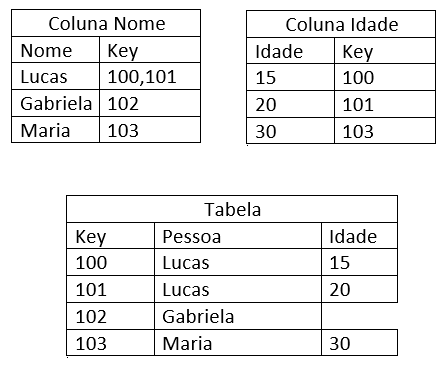
\includegraphics[width=0.4\textwidth]{./04-figuras/db-colunar}
    \fonte{O Autor}
    \label{fig:db-colunar}
\end{figure}


Cada modelo de dados possui suas vantagens e desvantagens, e a melhor escolha depende do que 
se deseja alcançar. Apesar das modelagens e SGBDs não relacionais possuirem claras vantagens,  
elas ainda possuem certas limitações. Por exemplo, a maioria das implementações NoSQL não
suportam as operações \textit{join} e \textit{order by} \cite{pokorny2013nosql}. 
Nesse contexto surgem outras plataformas, para auxiliar no processamento de grandes volumes 
de dados, e que possuem uma comunicação natural com bancos de dados NoSQL. Na próxima seção 
são apresentadas duas dessas plataformas, o Hadoop e o Spark.

\section{Hadoop e Spark}
\label{sec:spark}

O Apache Hadoop\footnote{http://hadoop.apache.org/}, também conhecido apenas como Hadoop, 
é um projeto de código aberto mantido pela Apache Software Foundation, que desenvolve 
softwares para processamento distribuído de grandes volumes de dados. O ecossistema do 
Hadoop é composto por quatro módulos:(1) \textit{Hadoop Common}, (2) 
\textit{Hadoop Distributed File System (HDFS)}, (3) \textit{Hadoop YARN} e (4) 
\textit{Hadoop Map Reduce} \cite{kumar2014apache}. 

O primeiro, \textit{Hadoop Common}, é um conjunto de utilitários que suporta os outros módulos
do Hadoop. O HDFS é um sistema de arquivos distribuído que permite o armazenamento de um 
grande volume de dados em diversos nodos de um \textit{cluster}. As grandes vantagens do HDFS 
são: a portabilidade, capacidade de armazenamento, o custo-benefício e a tolerância a falhas. 

O YARN é um \textit{framework} para agendamento de tarefas e gerenciamento de recursos em 
\textit{cluster}. Por fim, o \textit{Hadoop MapReduce} é um método para distribuir tarefas 
em múltiplos nodos, o que permite o processamento paralelo e distribuído, tolerante a 
falhas e de fácil abstração. Como o próprio nome sugere, ele é baseado no \textit{MapReduce}, 
um modelo de programação e \textit{framework} introduzido pelo Google \cite{kumar2014apache}. 
A grande desvantagem do Hadoop é que seu processamento ocorre em disco, o que limita sua 
velocidade \cite{shoro2015big}.

Já o Apache Spark\footnote{http://spark.apache.org/}, ou simplesmente Spark, é uma ferramenta 
de propósito geral para processamento em \textit{cluster}, que realiza operações em memória. 
Esta característica permite o aceleramento da análise de dados, tornando mais rápido, 
tanto as operações de escrita quanto o processamento de dados. Em alguns casos o Spark pode ser 
até cem vezes mais rápido que o Hadoop. Além disso, o Spark possui APIs para diversas 
linguagens de programação, como Python, Java, Scala e R. Outra vantagem, é a existência de 
diversas ferramentas de alto nível que auxiliam no processamento de dados, como por exemplo 
a M Lib, uma biblioteca para aprendizado de máquina e o Spark SQL, uma biblioteca que 
permite, entre outras coisas, a realização de operações como \textit{join} e 
\textit{order by} em qualquer conjunto de dados, mesmo aqueles originários de bancos de 
dados NoSQL \cite{shoro2015big}.

Assim, dada uma fonte de dados NoSQL é possível utilizar o Hadoop ou Spark para acessar,
processar e até mesmo alimentar essa fonte. Por fim, deve-se permitir o acesso aos dados
já processados que são armazenados, isso pode ser realizado utilizando \textit{web services}. 


\section{\textit{Web Services}}
\label{sec:api}

A troca de informações entre aplicações distribuídas na web é feita através de protocolos de 
comunicação \cite{schepke2010avaliaccao}. Estes protocolos permitem, entre outras operações, a 
recuperação de dados de aplicações que possuem esse acesso liberado. Serão discutidos duas 
das formas de comunicação, conhecidas como \textit{web services}, mais utilizadas, o 
\textit{Simple Object Access Protocol (SOAP)}, e o \textit{Representational State 
Transfer (REST)} \cite{lima2012}.

O SOAP é um protocolo adotado pela W3C, que permite invocar aplicações remotas independente de 
linguagem de programação e plataforma. O protocolo é baseado em XML, e utiliza o 
\textit{Hypertext Transfer Protocol (HTTP)} para transporte da mensagem. Uma mensagem SOAP é 
composta por três elementos: (1) envelope, (2) cabeçalho e (3) corpo \cite{suda2003soap}.

O envelope SOAP é o recipiente que armazena os outros elementos da mensagem, como o cabeçalho 
e o corpo.  O cabeçalho é um elemento opcional, que contém informações adicionais, como por 
exemplo, se a mensagem deve ser processada por um nó intermediário antes de chegar ao ponto 
final da aplicação. O corpo SOAP é um elemento obrigatório, que armazena os dados da mensagem 
transportada. No caso de uma mensagem de requisição, o corpo pode conter o método a ser 
chamado e os parâmetros de entrada e saída do método, já para uma mensagem de resposta o 
corpo contém o resultado (dados), gerado pelo método chamado \cite{suda2003soap}.

O modelo REST foi definido por \citeonline{fielding2000architectural}, que buscou as melhores 
práticas de arquiteturas de \textit{web services} já existentes e compôs uma nova arquitetura 
que as reunissem em apenas uma. Essa arquitetura reúne as melhores práticas no que se refere 
a: (1) cliente/servidor, (2) sistemas de camadas, (3) cache e (4) sem estado 
\cite{fielding2000architectural}.

No modelo REST são definidos dois papéis, cliente e servidor. O servidor oferece uma série 
de serviços do qual o cliente faz uso. Ao receber uma requisição do cliente o servidor decide 
o que fazer com ela, aceitar a requisição ou rejeitá-la \cite{fielding2000architectural}.

Outra característica do modelo REST é a divisão em camadas. O sistema é dividido de forma que 
uma camada inferior conhece apenas a interface da camada superior, isso melhora a 
escalabilidade do sistema, mas adiciona uma sobrecarga no tratamento dos dados, o que pode 
ser combatido utilizando cache \cite{fielding2000architectural}. 

O cache evita que dados, que já tenham sido enviados anteriormente, sejam reenviados, isso 
melhora a eficiência, escalabilidade e performance dos servidores. Finalmente, o sistema 
não possui estado, ou seja, as informações para atender uma requisição estão contidas nela 
mesma \cite{fielding2000architectural}.

Diferentemente do SOAP, os \textit{web services} REST não possuem um formato padrão para envio 
de mensagens, os mais comuns são o JSON e XML. Além disso, a arquitetura REST utiliza o 
protocolo HTTP e seus métodos para manipulação de recursos. O termo recursos se refere a 
qualquer estrutura que pode ser armazenada em um computador. Esses métodos permitem, entre 
outras operações, a exclusão, atualização, inserção e recuperação de recursos \cite{lima2012}.

A desvantagem do serviço SOAP é o uso limitado do protocolo HTTP, já que utilizam um único 
método para realizar múltiplas operações, enquanto serviços REST utilizam todos os métodos 
disponíveis. Outra desvantagem do SOAP é a falta de flexibilidade na definição do formato 
das mensagens. No entanto, embora os serviços REST sejam mais flexíveis isso também pode ser 
um problema, já que em serviços flexíveis a interoperabilidade pode ficar prejudicada. Não 
existe serviço melhor que o outro, a escolha deve ser feita de acordo com o contexto 
\cite{lima2012}.